
\section{Classificador \textsc{KNN}.}
\label{subsec::cred_knn}

%No decorrer dessa seção, explicaremos o algoritmo dos K vizinhos mais próximos (do inglês, \textit{K-Nearest Neighbor}, KNN). Da mesma forma que fizemos com o \textit{Naïve Bayes}, dedicamos uma seção, Seção~\ref{subsubsec::knn_cred}, exclusivamente para abordarmos o \textsc{KNN} integrado a credibilidade. 

O algoritmo dos $K$ vizinhos mais próximos (\textsc{KNN}) é conhecido por ser um método de aprendizado baseado em analogias, ou seja, comparamos o teste com os exemplos contidos no treinamento a fim de conseguirmos encontrar aqueles com maior semelhança. 
Tipicamente, cada exemplo existente é uma tupla de $D$ dimensões e representa um ponto em um espaço $D$-dimensional. 
Quando um novo exemplo de teste necessita ser classificado, o algoritmo \textsc{KNN} procura nesse espaço $D$ dimensional pelos $k$ exemplos do treinamento que estão mais perto do teste. 
Por fim, os $k$ vizinhos mais próximos realizam uma votação para escolherem qual será a classe que o teste pertence.

Na Figura~\ref{fig::knn}, mostramos um triângulo que representa o exemplo de teste, além de quadrados e losangos, representando os exemplos de treinamento pertencentes as classes \textit{Quadrado} e \textit{Losango}, respectivamente. As órbitas circulares existentes na figura são epicêntricas e servem apenas para fins didáticos.
Por essa figura, vemos a importância do parâmetro $k$ na decisão da classe que um exemplo pertence. Considerando que cada exemplo tem o mesmo peso na votação, caso $k=1$, escolhemos a classe \textit{Losango} para o exemplo de teste, entretanto, se $k=5$, escolhemos a classe \textit{Quadrado}. Para valores de $k$ entre 2 e 4, como temos 3 vizinhos a uma mesma distância, necessitamos de algum método de desempate. Em nosso trabalho, ordenamos os vizinhos primeiramente pela distância até o teste e depois por um identificador único. Estamos condicionados a ordem dos identificadores como critério de desempate, o que não tem nenhuma semântica, mas é necessário definir. %Dessa forma, minimizamos problemas relativos a ordem como os exemplos de treinamento são apresentados.

\begin{figure}[ht!]
\centering
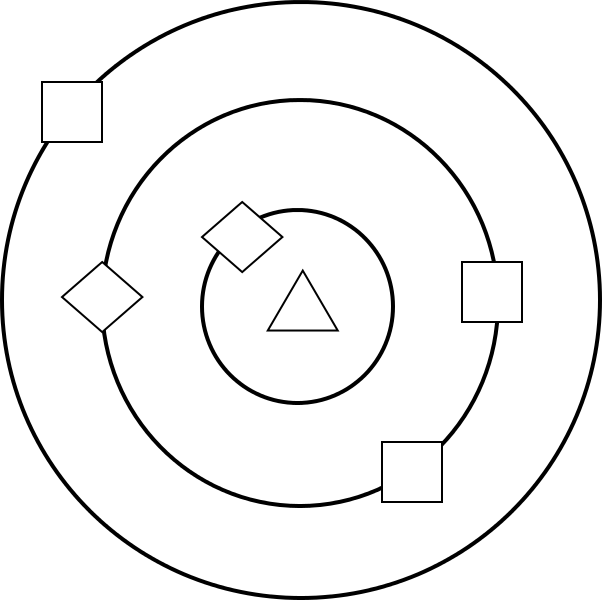
\includegraphics[width=0.5\textwidth]{figures/knn.png}
\caption{O algoritmo dos $k$ vizinhos mais próximos.}
\label{fig::knn}
\end{figure}

Como vimos, uma parte fundamental do \textsc{KNN} é podermos calcular o quão próximo um exemplo de teste está dos de treinamento. 
Essa proximidade é tipicamente calculada por uma métrica de distância que pode variar de problema para problema. Utilizamos 3 métricas diferentes, dependendo se estamos classificando um atributo $A_i$ que seja categórico, numérico ou textual. Para dois exemplos $X_1 =  (x_{11}, x_{21}, x_{31}, ..., x_{D1})$ e $X_2 = (x_{12}, x_{22}, x_{32}, ..., x_{D2})$, nos quais $x_{ij}$ representa o valor do atributo $A_i$ para o exemplo $j$, temos que, caso $A_i$ seja:

\begin{itemize}

\item Numérico, utilizamos a distância Euclidiana:

\begin{equation}\label{eqn::distancia_euclidiana}
    dist(X_1, X_2) =  \sqrt{\sum_{i=1}^D (x_{i1}-x_{i2})^2}
\end{equation}

    Com o intuito de evitar que um atributo com grande escala de valores sobreponha um outro atributo de uma menor escala, empregamos a normalização \textit{min-max} para todos os valores $x_i$ do correspondente atributo $A_i$: 

\begin{equation}\label{eqn::distancia_euclidiana}
    x'_{i} =  \frac{x_{i} - min_{A_i}}{ max_{A_i} - min_{A_i} }
\end{equation}

\item Categórico, comparamos $X_1$ e $X_2$ e somamos uma unidade a distância entre os exemplos para cada $x_i$ que tenha valores distintos entre $X_1$ e $X_2$.

\begin{equation}\label{eqn::distancia_cat}
   dist(X_1, X_2) = \sum_{1 < i < D \ \wedge \ x_{i1} \neq x_{i2}} 1.0
\end{equation}

\item Textual, tomamos a distância dos cossenos entre os dois exemplos $X_1$ e $X_2$ e invertemos o seu sinal. Ou seja, sendo $||X_j|| = \sqrt{ (x_{1j} \cdot w_{1j})^2 + (x_{2j} \cdot w_{2j})^2 + (x_{3j} \cdot w_{3j})^2 + ... + (x_{Dj} \cdot w_{Dj})^2}$ a norma do vetor representado por um exemplo $X_j$ no espaço, $x_{ij}$ como a frequência do peso de um termo $A_i$ no documento $j$ e $w_{ij}$ representando o peso referente ao atributo $A_i$ no documento $j$, temos que a semelhança entre dois exemplos $X_1$ e $X_2$ pode ser definida como:

\begin{equation}\label{eqn::distancia_texto}
    cosSim(X_1, X_2) = \sum\limits_{1 < i < D} \frac{ x_{i1} \cdot w_{i1} \cdot x_{i2} \cdot w_{i2} }{ ||X_1|| \cdot ||X_2|| }
\end{equation}

Primeiro, cabe explicar que usamos a métrica \textsc{IDF} (\textit{inverse document frequency}, Seção~\ref{sec::pg_cred_baseada_conteudo}), como o peso $w_{ij}$ do termo $A_i$ no documento $j$. Segundo que, como dito, a métrica acima é chamada de semelhança dos cossenos por se basear no ângulo cosseno entre dois vetores no espaço. Como observado, estamos interessados na métrica inversa, logo:
 
 \begin{equation}\label{eqn::distancia_texto2}
    dist(X_1, X_2) = - cosSim(X_1, X_2)
\end{equation}


\end{itemize}

Note que após calcularmos a distância entre o exemplo de teste e os exemplos de treino, realizar uma votação entre os $k$ vizinhos mais próximos é um processo muito simples. Basta contabilizar os votos de cada um dos $k$ vizinhos e atribuir ao exemplo de teste a classe vencedora.

\section{Incorporando a Credibilidade ao \textsc{KNN}.}
\label{subsubsec::knn_cred}

Realizamos nessa seção um paralelo ao feito na discussão sobre o \textit{Naïve Bayes} nas Seções \ref{subsubsec::nbcredatributos} e \ref{subsubsec::nbcredgrafos}. Portanto, iremos discutir como incorporar ao \textsc{KNN} a credibilidade baseada nos atributos dos exemplos na Seção \ref{subsubsec::knncredatributos} e aos relacionamentos na Seção~\ref{subsubsec::knncredgrafos}.
%, analisaremos a credibilidade do ponto de vista das interações entre o exemplo de teste e os exemplos de treinamento, modeladas por meio de grafos.

\subsection{\textsc{KNN} com Credibilidade Baseada nos Atributos.}
\label{subsubsec::knncredatributos}


Acoplamos a credibilidade ao algoritmo \textsc{KNN} de forma bem semelhante ao que fizemos com o \textit{Naïve Bayes}. 
Novamente, buscamos uma maneira de quantificar o relacionamento entre um atributo e uma classe. 
Note que o \textsc{KNN} não realiza essa associação explicitamente, ou seja, como vimos na Seção~\ref{subsec::cred_knn}, somente observamos a classe pertencente a um exemplo de treinamento quando já temos os $k$ vizinhos mais próximos definidos, então realizando uma votação para saber qual a classe a ser escolhida.

O \textsc{KNN} é um algoritmo que, de uma maneira geral, compara dois exemplos, um do conjunto de teste e outro do de treino, e se baseia em algum cálculo respectivo a um mesmo atributo $A_i$ de cada um dos exemplos para calcular a distância entre eles. Dessa vez, fica bem claro que alteramos a distância entre dois exemplos ao usar a credibilidade baseada nos atributos. 
%O que tentamos fazer é aproximar o quanto de credibilidade tem a informação que o exemplo de teste pertence a mesma classe do exemplo de treino, sendo que o atributo $A_i$ tem valor $x_i$ e utilizar essa informação para melhorar o \textsc{KNN}.
%é utilizar o conhecimento da classe a qual o exemplo de treino pertence e avaliarmos o 

No algoritmo \textsc{KNN}, a fórmula da distância entre dois exemplos muda drasticamente dependendo do tipo dos atributos.
Efetivamente, em nossos testes, empregamos a credibilidade para classificação textual e categórica. Embora acreditemos que seja perfeitamente possível utilizarmos o mesmo raciocínio para definirmos a credibilidade em atributos numéricos, deixamos essa tarefa como trabalho futuro. A seguir, nas Seções~\ref{subsubsec::knncat} e~\ref{subsubsec::knntexto}, apresentamos as modificações realizadas no algoritmo dos $k$ vizinhos mais próximos para os atributos categóricos e textuais, respectivamente.

\subsubsection{\textsc{KNN} Categórico.}
\label{subsubsec::knncat}

Procuramos, ao desenvolver as modificações seguintes, ter em vista dois fatos importantes:
\begin{enumerate}
\item Se o exemplo de treinamento e o de teste têm os mesmos valores para todos os seus atributos, então a distância entre eles é zero. 
\item Um exemplo de treino que apresenta diferença em $T$ atributos do exemplo de teste, tende a ter uma distância menor que outro que apresente $T+1$ atributos distintos.
\end{enumerate}

A regra 1 é bastante intuitiva. A regra 2 diz que, ao levar em consideração a credibilidade do exemplo de treinamento, criamos uma mudança no espaço de atributos. Porém, queremos que essa mudança seja controlada. Ou seja, a hipótese básica do \textsc{KNN} de que exemplos parecidos (com grande número de atributos iguais) estão bem próximos em uma distribuição espacial deve ser respeitada.

Visualmente, o que queremos com a modificação realizada no algoritmo dos vizinhos mais próximos está expresso na Figura~\ref{fig::KNNantesedepois}. Na Figura~\ref{fig::KNNantesedepois}-(a) temos a situação já discutida anteriormente, composta de um exemplo do treino que difere em uma característica, três que diferem em duas e um outro que difere em três, sendo que esses são os cinco vizinhos mais próximos de nosso exemplo de teste. Por sua vez, na Figura~\ref{fig::KNNantesedepois}-(b) temos os mesmos exemplos mostrados, porém com as distâncias entre o teste e o treino sendo comparadas utilizando a credibilidade de que o exemplo de teste pertence a cada uma das classes dos exemplo de treino. 
Pode-se observar que os exemplos da classe \textit{Losango} foram mais afetados, o que pode significar que o exemplo de teste pertence a essa classe. Dessa vez, ao contrário do que temos na situação anterior, para valores de $k$ entre 1 e 3, sabemos definir que o teste pertence a classe dos losangos, sem precisarmos utilizar uma métrica especial de desempate. 

\begin{figure}[ht]
\centering
\subfloat[\textsc{KNN} original]{
    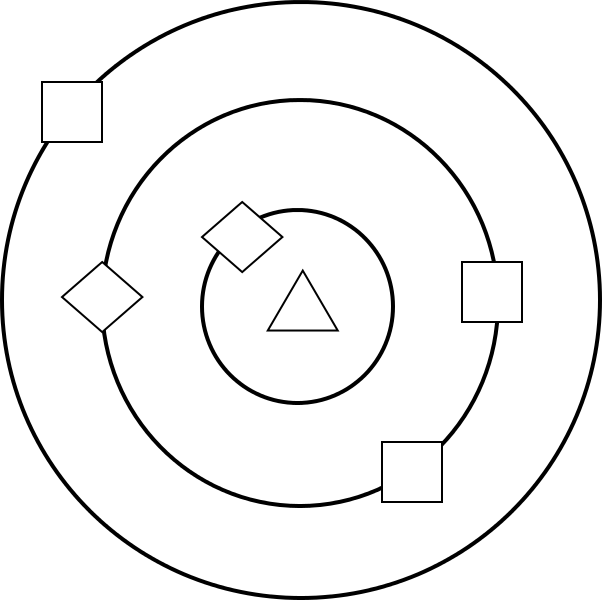
\includegraphics[width=0.5\textwidth]{figures/knn.png}
}
\subfloat[\textsc{KNN} com credibilidade]{
%    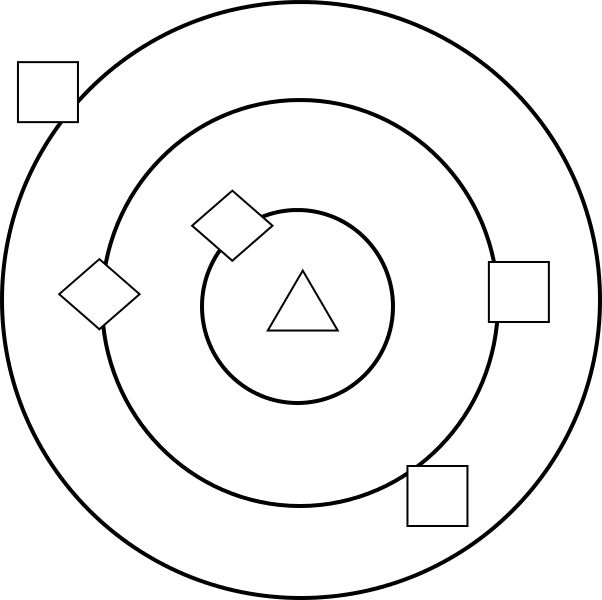
\includegraphics[width=0.5\textwidth]{figures/knncred.png}
    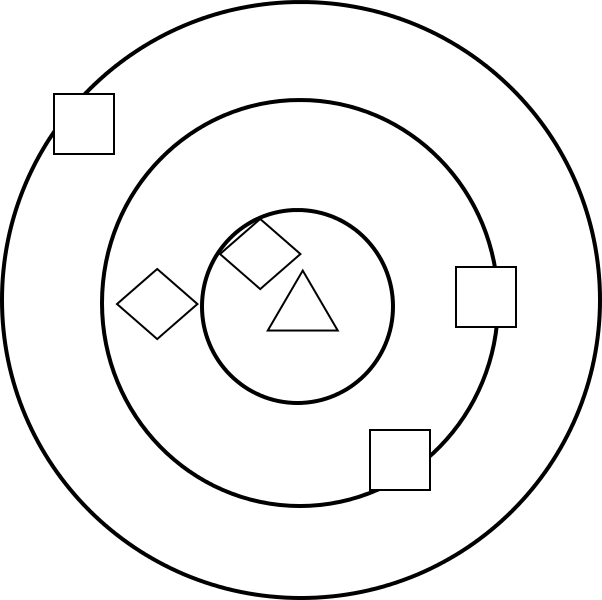
\includegraphics[width=0.5\textwidth]{figures/knn_aproxima.png}
}
\caption{Em (a) temos o algoritmo original dos $K$ vizinhos mais próximos e em (b) temos um possível resultado da utilização da credibilidade conjuntamente ao \textsc{KNN}.  
\label{fig::KNNantesedepois}}
\end{figure}

Levando em consideração o que foi mostrado até esse ponto, sendo $X_1$ o exemplo de teste, $X_2$ o de treino e $c_{X_2}$ a classe a qual $X_2$ pertence, modificamos a Equação~\ref{eqn::distancia_cat} para:

\begin{equation} \label{eqn::distancia_cat_cred}
   dist(X_1, X_2) = \sum_{1 < i < D\ \wedge \ x_{i1} \neq x_{i2}} \frac{1.0}{1.0 + Cr_{atr}(x_{i1}, c_{X_2} ))}
\end{equation}

Adicionamos um termo relacionado a credibilidade na Equação~\ref{eqn::distancia_cat}, um fator inversamente proporcional ao valor calculado para a credibilidade. Note que como definimos a credibilidade como sendo sempre um valor positivo, a distância entre $X_1$ e $X_2$ será sempre menor ou igual a uma unidade, sendo que, quanto menor ela for, maior a credibilidade. 
%Caso não somarmos o primeiro termo 1.0 na equação acima, então teríamos valores entre zero e um para a distância, onde maiores valores para a credibilidade estariam mapeados para distâncias próximas a zero e valores baixos para distâncias próximas a um. Ambos métodos são perfeitamente compatíveis, porém para ilustrar o que foi definido e modelado na Figura~\ref{fig::KNNantesedepois} é necessário somar o fator 1.0. 
%Para garantirmos o efeito mostrado na Figura \ref{fig::KNNantesedepois}, adicionamos um termo relacionado a credibilidade na Equação~\ref{eqn::distancia_cat}, um fator inversamente proporcional ao valor calculado para a credibilidade. Note que como definimos a credibilidade como sendo sempre um valor positivo, teremos que a distância entre $X_1$ e $X_2$ é sempre maior que uma unidade, sendo que maior ela será quando menor for a credibilidade. Caso não somarmos o primeiro termo 1.0 na equação acima, então teríamos valores entre zero e um para a distância, onde maiores valores para a credibilidade estariam mapeados para distâncias próximas a zero e valores baixos para distâncias próximas a um. Ambos métodos são perfeitamente compatíveis, porém para ilustrar o que foi definido e modelado na Figura~\ref{fig::KNNantesedepois} é necessário somar o fator 1.0. 


\subsubsection{\textsc{KNN} Textual.}
\label{subsubsec::knntexto}

Assim como feito na incorporação da credibilidade nos atributos categóricos, utilizamos a informação da classe do exemplo de treino para aferir a credibilidade daquele exemplo em relação àquela classe. Sendo $t_i$ o termo referente ao atributo $A_i$, $x_i$ a frequência do mesmo e $w_i$ o seu peso (como já explicado, usamos a métrica \textsc{IDF}), adaptamos a Equação~\ref{eqn::distancia_texto}, como:

\begin{equation}\label{eqn::distancia_texto_cat}
    dist(X_1, X_2) = \sum\limits_{1 < i < D}\frac{  Cr_{atr}(t_{i1}, c_{X_2}) \cdot x_{i1} \cdot w_{i1} \cdot x_{i2} \cdot w_{i2} }{ ||X'_1|| \cdot ||X_2|| }
\end{equation}

Repare que utilizamos $||X'_1||$ como a norma do vetor $X_1$, levando em conta a credibilidade em relação à classe do exemplo de treino $X_2$, logo temos que $||X'_1|| = \sqrt{ ( Cr_{atr}(x_{11}, c_{X_2}) \cdot x_{11} \cdot w_{11} )^2 + ... +  ( Cr_{atr}(x_{D1}, c_{X_2}) \cdot x_{D1} \cdot w_{D1} )^2}$.

Novamente, assim como discutido na Seção~\ref{subsubsec::nbcredatributos}, existem diversas métricas que podemos utilizar para inferirmos a credibilidade de um elemento, a fim de melhorarmos a classificação do algoritmo \textsc{KNN}. Elas serão discutidas no Capítulo~\ref{cap::metodo}.
%Algumas dessas métricas já foram previamente discutidas e o serão novamente ao longo desse trabalho. Entretanto, voltamos a frisar que a escolha de uma função de credibilidade é dependente ao contexto que a mesma está inserida e combinar as métricas disponíveis é uma tarefa combinacional cara e, para tanto, estamos usando Programação Genética como será discutido em detalhes no Capítulo~\ref{cap::programacao_genetica}.

\subsection{\textsc{KNN} com Credibilidade Baseada em Relacionamentos.}
\label{subsubsec::knncredgrafos}

A mesma situação exposta com detalhes na Seção~\ref{subsubsec::nbcredgrafos} retoma à cena. Modelamos a credibilidade existente nos relacionamentos entre um exemplo de teste e uma classe, baseando nos exemplos do treino. 
%tribuída a um exemplo de teste em relação a determinada classe utilizando o relacionamento que aquela instância tem com as demais instâncias de treino, levando em consideração a classe que as mesmas pertencem.
Diferentemente da modelagem da credibilidade para o conteúdo do algoritmo \textsc{KNN}, dessa vez podemos criar apenas um modelo que se adapta a qualquer tipo de atributo numérico, categórico ou textual. Logo, sendo $R$ o número de relacionamentos modelados, $X_1$ o exemplo de teste, $X_2$ o exemplo de treino e $\alpha$ o fator somado a credibilidade dos relacionamentos para evitarmos valores nulos no denominador, temos:

\begin{eqnarray}\label{eqn::distancia_grafos}
    dist(X_1, X_2) & = & \frac{ dist(X_1, X_2) } { \alpha + Cr_{rel}(X_1, class_{X_2}) }\\
    Cr_{rel}(X, c_j) & = & \prod^{R}_{i=1} {Cr_{i}(X,c_j)} 
\end{eqnarray}

%Note que estamos modificando o valor da distância calculado entre o exemplo de teste e os de treino, baseando no fato que quanto maior a credibilidade do relacionamento do teste $X_1$ a uma classe $c_i$, menor será a distância entre o exemplo $X_1$ e os outros exemplos do treinamento que pertencem a classe $c_i$.
Note que quanto maior a credibilidade do relacionamento do teste $X_1$ a uma classe $c_i$, menor será a distância entre o exemplo $X_1$ e os exemplos do treino que pertencem a classe $c_i$, exatamente como modelado para o \textit{Naïve Bayes}.

Mais uma vez, podemos utilizar as várias propriedades dos grafos para calcularmos a credibilidade dos relacionamentos. Na Seção~\ref{sec::pg_cred_baseada_grafos}, definimos várias métricas que calculam essas propriedades. 
%Por fim, usamos a Programação Genética para combinar essas métricas a fim de obtermos uma melhor função de credibilidade que explore melhor o relacionamento exemplo-classe.

